% -*- root: ../main.tex -*-
\chapter{Piano di lavoro}
Il lavoro è stato svolto utilizzando un approccio Scrum, con quattro sprint, più uno iniziale incentrato sullo studio delle tecnologie.
\section{Contributi}
Di seguito vi è una descrizione delle mansioni che sono state svolte dai membri del gruppo.
\paragraph{Sara Kiade} 
\begin{itemize}
    \item progettazione e realizzazione del database
    \item implementazione logiche di interrogazione e calcolo nel back-end della Web-App
    \item implementazione e testing delle funzioni nel front end 
    \item stesura template delle funzioni nel back-end
    \item configurazione SAM
    \item prototyping della sensoristica
    \item realizzazione diagrammi sequenza
\end{itemize}

\paragraph{Gyordan Caminati}
\begin{itemize}
    \item implementazione del front-end
    \item integrazione nelle adeguate pagine del front-end delle chiamate al backend 
    \item configurazione SAM
    \item implementazione di alcune funzioni nel backend
    \item scheduling di funzioni lambda innescate da Crono Cloud Watch, MQTT, Api Gateway
    \item implementazione scheduler Micropython
    \item prototyping della sensoristica
    \item realizzazione diagrammi sequenza
\end{itemize}
\paragraph{Igor Lirussi}
\begin{itemize}
    \item implementazione scheduler Micropython
    \item implementazione funzioni core di Micropython e classi per sensori/attuatori
    \item implementazione sistema di videosorveglianza con motion detecion e object detection
    \item implementazione script di automatizzazione caricamento file
    \item prototyping della sensoristica
    \item progettazione e implementazione macchina a stati 
\end{itemize}
La collocazione temporale degli sprint è descritta nel seguente diagramma di Gantt: 
\begin{figure}[H]
    \caption{Gantt Chart del progetto}
    \label{fig:Gantt}] 
    \centering
   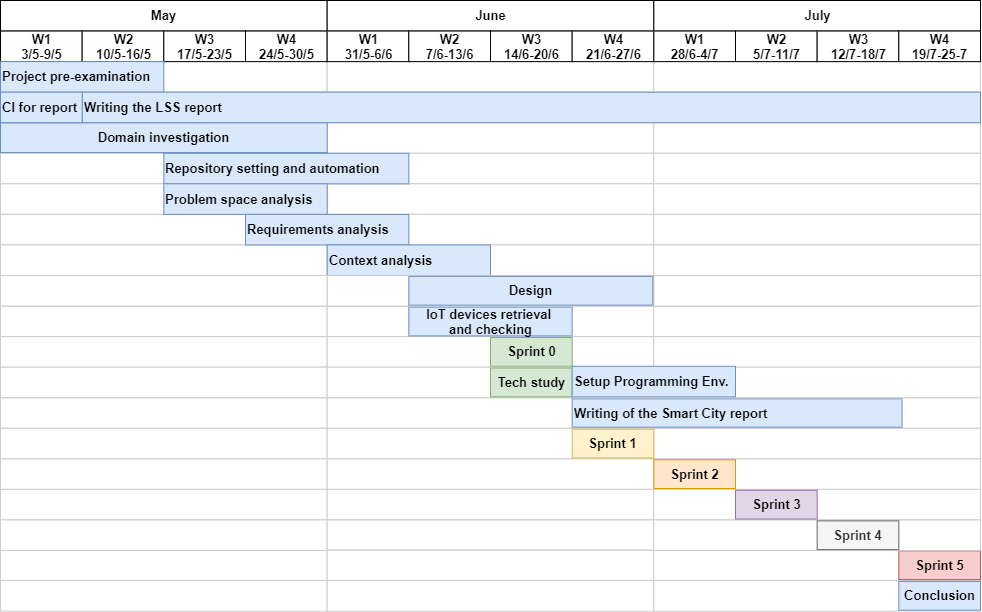
\includegraphics[width=1\textwidth]{DrawIo/GanttChart.png}
\end{figure}

\section{Svolgimento}
Gli sprint sono stati portati avanti nel seguente modo:
    \paragraph{Sprint Planning}
        Pianificazione a inizio sprint degli obiettivi, tempistiche e responsabilità nel periodo dello sprint corrente. Diviso in due parti:
        \begin{itemize}
        \item\textbf{parte 1} 
            Viene raffinato e rivisto il product backlog, viene effettuata la scelta dello sprint goal (what).
        \item\textbf{parte 2}
            Si decidono gli item e viene raffinato come implementarli (how). Effettuato con solo il team senza la figura del product owner
        \end{itemize}
    \paragraph{[Iterativo] Daily scrum} Breve meeting svolto giornalmente. Viene utilizzato per gli aggiornamenti sull'andamento del progetto, senza scendere nei dettagli implementativi.
    \paragraph{[Occasionale] Pair Programming } Utilizzato per risolvere problemi che causano il blocco di un componente del team per parecchio tempo su una issue.
    \paragraph{Meeting finale}
        Riflessioni e considerazioni finali sullo spint passato. Suggerimenti per migliorare il prossimo. Diviso in tre parti: 
        \begin{itemize}
        \item\textbf{Product backlog refinement} aggiunta di dettagli e riordino del product backlog
        \item\textbf{Sprint review} è stato ispezionato l'incremento, il Minimum Viable Product o di risultati sul processo. Discernere cosa è stato fatto e cosa no
        \item\textbf{Retrospettiva} Considerazioni sul team stesso e sui miglioramenti per il prossimo sprint. 
        \end{itemize}
        
        

\section{Sprint 0}
All'interno dello sprint 0 il focus è stato sullo scegliere le giuste tecnologie di sviluppo e sull'apprenderle in maniera sufficiente per il kick-off del progetto.
L'obiettivo è stato raggiungere una conoscenza e competenza minima per sviluppare il design in maniera consapevole e ottimale.
\paragraph{Deliverables} 
al termine di questo sprint si sono acquisite le competenze di base per poter iniziare a lavorare con AWS e i dispositivi IoT. Inoltre ci si è portati avanti con lo scheletro del sito.
\begin{itemize}
    \item ambiente di lavoro Linux standardizzato e virtualizzato
    \item sito linkato, con le prime due pagine base: home e login
    \item ESP32 con firmware installato MicroPython, script e guida all'uso
    \item codice per sensori base, test relativi e stubs per eseguirli senza necessità del micro-controllore
    \item repository software con CI e test automatizzati 
    \item database progettato e popolato con qualche dato ai fini di testing
\end{itemize}

\section{Sprint 1}
All'interno dello sprint 1 il focus è stato sull'usare le competenze tecnologiche acquisite precedentemente per sviluppare i componenti principali del progetto. Sono stati scelti come obiettivi le user stories per l'automatizzazione di cibo e acqua e la visualizzazione delle informazioni relative a un animale sulla webpage.
\paragraph{Deliverables}
al termine di questo sprint sono state implementate le funzioni base dei maggiori componenti per l'automatizzazione fisica di cibo e acqua e il relativo prototipo fisico. Sono state aggiunte sull'applicativo la vista delle informazioni dell'animale e l'impostazione del cibo da erogargli. 
\begin{itemize}
    \item codice per i sensori/attuatori per acqua e cibo, con stubs, test e automatizzazione. (Livello acqua, elettrovalvola, motore, bilancia, laser e rilevatore di luce)
    \item prototipo fisico per i sensori per acqua e cibo. 
    \item database migliorato e rifattorizzato
    \item visualizzazione dei dati del cane sul sito 
    \item visualizzazione dei grafici delle statistiche sul sito 
\end{itemize}

\section{Sprint 2}
Nello sprint 2 il focus è stato sul realizzare la logica d'orchestrazione della sensoristica e l'integrazione tra essa e l'applicativo per mezzo del protocollo MQTT. Sono stati prodotti gli artefatti di documentazione e schemi esemplificativi. Inoltre, è stato dato peso alla creazione delle query che permettono di integrare le funzioni del sito con il database. In particolare ci si è concentrati sulle user-stories prioritarie, che costituiscono il core del dominio.
\paragraph{Deliverables}
\begin{itemize}
    \item sviluppate query necessarie alla logica centrale dell'applicazione web
    \item grafici per la temperatura e l'umidità nell'applicazione web
    \item implementata coverage dei test Python, con relativa pagina web su Github pages. 
    \item aggiunta Quality Assurance con SonarCloud, Codacy e Codefactor
    \item implementata Continuous Delivery con GitHub Actions e GitHub Releases
    \item implementata macchina a stati per food delivery e water automation
\end{itemize}

\section{Sprint 3}
Nello sprint 3 sono state implementate le query che verranno chiamate dal sito per mostrare gli elementi all'utente. Inoltre, è stato migrato il codice JavaScript in un repository dedicato che permette il deployment delle funzioni in automatico su AWS con SAM. Sono state sviluppate le funzioni per ottenere i dati della sensoristica del collare smart, implementando la logica per il controllo dei valori e l'invio delle notifiche su MQTT.
\paragraph{Deliverables}
\begin{itemize}
    \item sviluppate query complesse necessarie alla logica centrale dell'applicazione web
    \item repository dedicato delle funzioni JavaScript per AWS
    \item setup framework SAM per automazione AWS
    \item prototipo fisico per i sensori di temperatura e battito
    \item implementata macchina a stati per smart-collar heartbeat e temperature
\end{itemize}

\section{Sprint 4}
Lo sprint 4 è stato il più impegnativo,  perché vi era la necessità di chiudere il progetto, portando a termine tutti i task preventivati.
Una grossa parte dello sprint è stata dedicata all'integrazione delle diverse parti, alla chiusura delle ultime interrogazioni al database, all'inserimento degli ultimi pezzi dell'interfaccia grafica che permettono all'utente di interagire con il back-end e alla conclusione del sistema di sorveglianza.
\paragraph{Deliverables}
\begin{itemize}
\item Completamento WebApp che permette all'utente di interagire con il sistema, visualizzando i dati e apportando delle modifiche. 
    \item Completamento Back-end che gestisce la logica del sito
    \item Completamento gestione di sensori, attuatori e sistema di sorveglianza.
\end{itemize}



